\section{Exploratory Data Analysis}
\label{sec:eda}

\subsection{Data description}
\label{subsec:description}

The provided dataset contains personal information of several people
(8164 samples), such as date of birth and current employment and maps
it to the observation if the person became unemployed in the next 12 months.

The dataset was made available without any information about it's contents
except for the property names.
Each one was analysed for insights and anomalies.

The following list details what could be obtained exploring the data
(column name, value types and values).

\begin{description}
\item [id] Integer, identifier for each subject, all values distinct no
    problems detected.

\item [target] Integer, did the subject become unemployed in the following
    12 months.

\item [birth date] Date (YYYY-MM-DD), date of birth of the subject.
    The youngest being \DTMdisplaydate{2016}{2}{10}{-1} and the oldest
    \DTMdisplaydate{1928}{01}{09}{-1}.
    Frequency plot (see \vref{fig:birth_date_freq}) shows nothing surprising.

\item [country of origin] Categorical, country names come in a variety of
    inconsistent formats.

\item [domestic relationship type] Categorical,
    (see \vref{tab:domestic_relationship_type_value_counts}) who the subject
    lives with.
    Categories are unclear and ill defined.
    Moreover it is inconsistent with the \emph{domestic status}, there are a
    considerable number of entries classified as
    \emph{domestic relation type}--\emph{never married} and
    \emph{domestic status}--\emph{d} (presumably divorced)
    (see \vref{tab:domestic_type_by_status_counts}).

\item [domestic status] Categorical, marital status or if has married several
    times (see \vref{tab:domestic_status_value_counts}).
    By elimination category \emph{d} is supposedly divorced.

\item [earned dividends] Numerical, monetary amount (currency not specified).
    Return from distribution of corporate earnings, it's 0 for all samples.

\item [ethnicity] Categorical, categories have funny names
    (see \vref{tab:ethnicity_value_counts}).

\item [gender] Categorical, all female dataset
    (see \vref{tab:gender_value_counts}).

\item [job type] Categorical, current job type of the subject
    (see \vref{tab:job_type_value_counts}), government, self employed,
    item etc\ldots

\item [interest earned] Numerical, monetary amount (currency not specified).
    Returns from loaning money (see \vref{fig:interest_earned_freq}).

\item [monthly work] Numerical, number of hours of work per month
    (see \vref{fig:monthly_work_freq})

\item [profession] Categorical, type of profession
    (see \vref{tab:profession_value_counts}).

\item [school level] Categorical, subject level of schooling
    (see \vref{tab:school_level_value_counts}).

\end{description}


\subsection{Data exploration}
\label{subsec:exploration}

To get some further insights from the data the correlation matrix was
inspected.
It was split in multiple plots to ease this process \vref{fig:cross-matrix}.
Some pre-processing was necessary to produce the correlation matrix
see \vref{sec:data} for a description.

Some insights were expected, for example, the categorical dummy variables
have a strong negative correlation between themselves.
These dummy variables are not independent which will present a challenge
to linear models (consider applying PCA if using linear models).
There is a strong (negative or positive) correlation between the \emph{target}
and the \emph{domestic status}--\emph{married 2},
\emph{domestic relationship type}--\emph{has husband}, which could be
interesting to explore.
Also as expected the \emph{birth date} is connected with the
\emph{domestic status} classes, the connection with \emph{school level} is
not evident.
Finally there are severall connections between specific \emph{countries of
origin} and \emph{school level} and \emph{ethnicity}.

To help understand the dataset we trained a small decision tree see
\vref{fig:decision-tree}.
Although the decision tree model does not give good results (see
\vref{sec:initialTests}) it is still interesting to observe what features
split the data.
In fact, this model with a \verb+max_depth+ of 4 we outperformed the same
model using the standard parameters obtaining a \(0.8927\) AUC ROC score.
But this is the maximum obtained using simple decision trees.

\begin{figure}[!h]
    \caption{Date of birth frequency.}
    \label{fig:decision-tree}
    \centering
    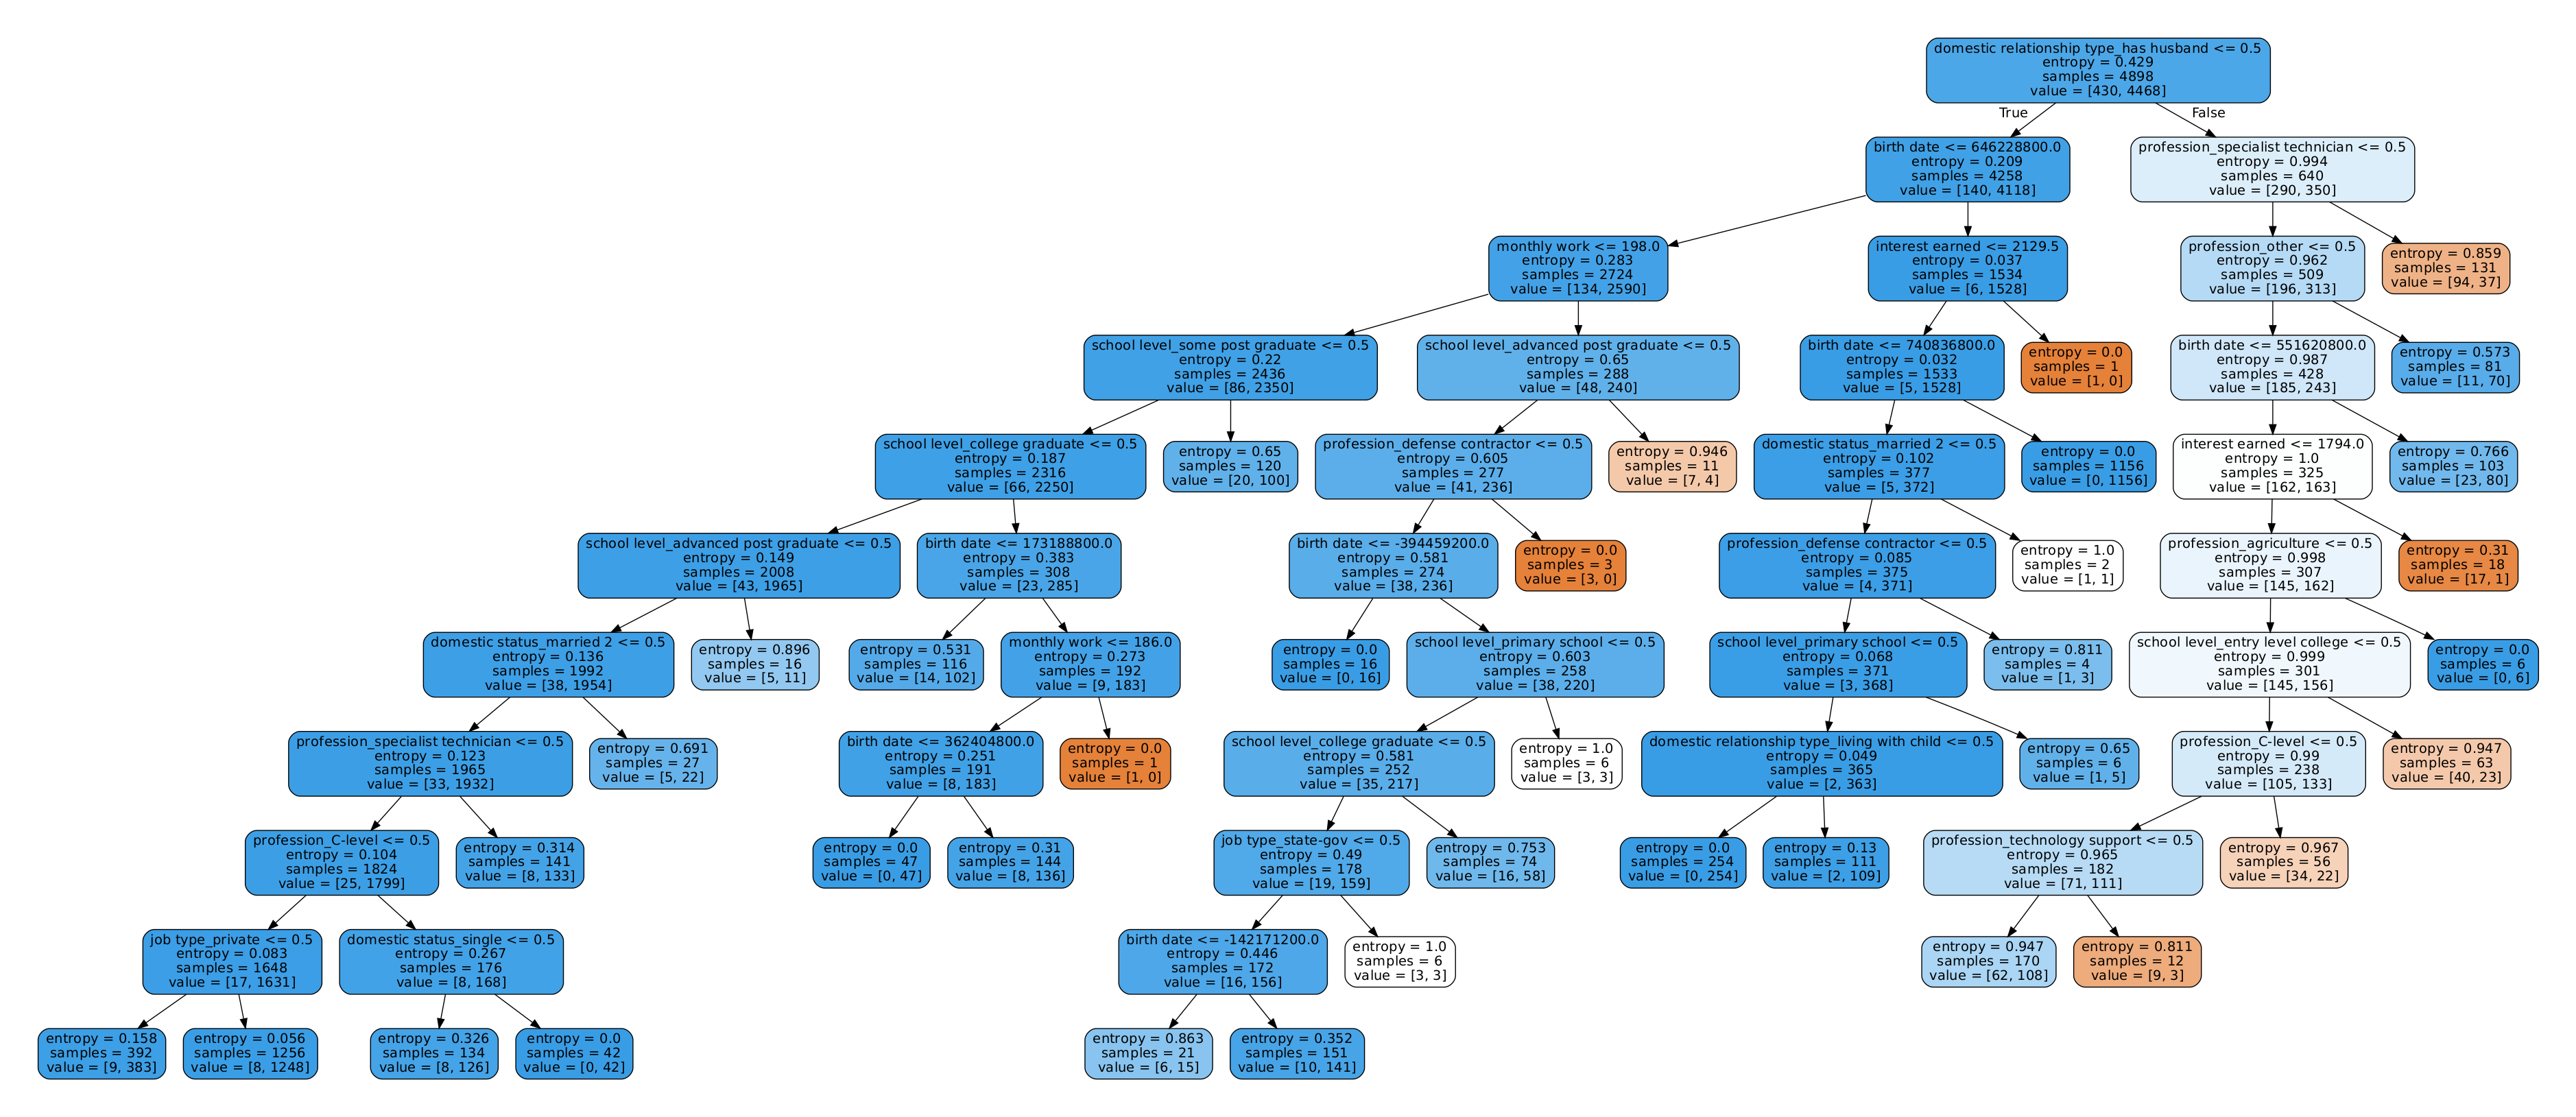
\includegraphics[width=\textwidth]{./img/decision-tree.png}
\end{figure}
